
\documentclass[conference]{IEEEtran}
\usepackage{graphicx}
\usepackage{amsmath}

\title{Classifying Sentiments in the Olist Reviews Dataset}

\begin{document}
\maketitle

\section{Dataset}
The dataset used in this analysis includes customer reviews and order data from the Olist e-commerce platform. 
We utilized two main files: \texttt{olist\_orders\_dataset.csv} and \texttt{olist\_order\_reviews\_dataset.csv}. 
After loading the data, the datasets were merged on the \texttt{order\_id} field to combine review data with associated orders. 
This dataset contains review scores, review messages, and other order-related fields.

\section{Classification Pipeline}
We implemented a Logistic Regression classifier to predict the sentiment (positive or negative) of customer reviews. 
The text data was preprocessed using stemming techniques (RSLP Stemmer), and vectorized using TF-IDF (Term Frequency-Inverse Document Frequency) to quantify the importance of each word.

A pipeline was constructed to automate these steps:
\begin{itemize}
    \item Text Preprocessing (Tokenization, Stemming)
    \item Vectorization (TF-IDF)
    \item Classification (Logistic Regression)
\end{itemize}

\section{Evaluation}
To evaluate the model's performance, we used several metrics:
\begin{itemize}
    \item Accuracy: Proportion of correctly classified reviews.
    \item Confusion Matrix: Visualization of predicted vs. actual classifications.
    \item Classification Report: Precision, Recall, and F1-Score for both classes.
\end{itemize}

\section{Dataset Size}
The dataset contains thousands of reviews, with the following distribution of review scores (5 stars being the highest, 1 star being the lowest). 
Figure~\ref{fig:review_distribution} shows the distribution of star ratings.

\begin{figure}[ht]
\centering
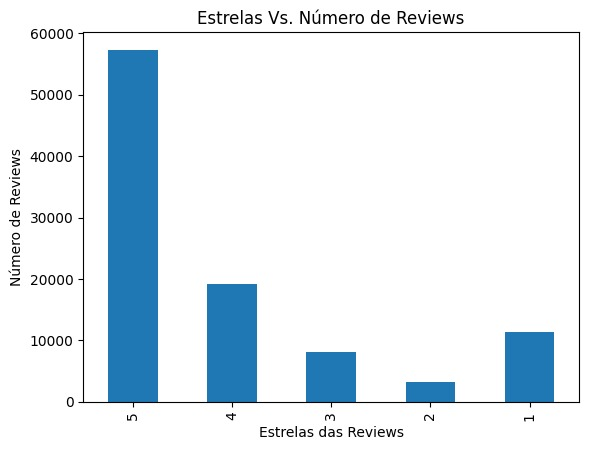
\includegraphics[width=0.45\textwidth]{review_distribution.png}
\caption{Distribution of Review Scores. The majority of reviews are concentrated on 5 and 4-star ratings, indicating positive feedback.}
\label{fig:review_distribution}
\end{figure}

\section{Topic Analysis}
A preliminary analysis of the reviews suggests common themes around customer satisfaction and product quality. 
Further topic analysis would allow the identification of frequent topics mentioned in positive and negative reviews.

\end{document}
